\section{Comparación de las abstracciones generadas entre el algoritmo clásico y el alternativo}
Como mencionamos en la sección \ref{sec:subaproximacion}, las abstracciones generadas por el algoritmo alternativo no siempre son Enabledness Preserving Abstractions\footnote{Es decir, en algunos casos no cumplen la definición presentada en la sección \ref{definicion-epa}.} de los contratos analizados, sino que son unas subaproximaciones de estas.
Al mismo tiempo, las EPAs son sobreaproximaciones del comportamiento de los contratos, por lo que el mecanismo resultante del algoritmo alternativo yace en algún lugar intermedio: no es ni sound ni complete.
Por esto, nos interesa explorar en particular cuáles son las diferencias producidas entre el algoritmo alternativo y las generadas por el algoritmo clásico (las EPAs) para evaluar su utilidad.
Para responder estas preguntas analizamos el desempeño de los prototipos implementados usando ambos algoritmos sobre algunos casos de prueba.

\subsection{Caso \texttt{RoomThermostat}}
El primer caso que evaluamos fue el contrato \texttt{RoomThermostat} perteneciente al benchmark ``Microsoft Azure Blockchain Workbench" \cite{azure-benchmark}, cuyo código fuente podemos ver en el fragmento de código \ref{fig:rooomthermostat-solidity}.
Es un contrato pequeño, con pocos métodos y un invariante sencillo.
Para poder emplear el algoritmo clásico sobre este contrato, el invariante propuesto fue el siguiente:
\begin{lstlisting}[language=Solidity]
    function invariant(StateType stateNew, address installerNew, address userNew, int targetTemperatureNew, ModeEnum modeNew) public returns(bool){
        bool result = (stateNew == StateType.Created || stateNew == StateType.InUse);
        result = result && (modeNew == ModeEnum.Auto || modeNew == ModeEnum.Cool || modeNew == ModeEnum.Heat || modeNew == ModeEnum.Off);
        if(stateNew == StateType.Created){
            result = (targetTemperatureNew == 70) && (modeNew == ModeEnum.Off);
        }
        return result;
    }
\end{lstlisting}

Luego, evaluamos tanto el algoritmo clásico como el alternativo sobre el contrato.
En ambos casos la EPA generada fue la misma, una máquina de estados sencilla de tan sólo tres estados que podemos ver en la figura \ref{fig:room-thermostat-epa}.

\begin{figure}
    \centering
    \begin{subfigure}{0.75\textwidth}
        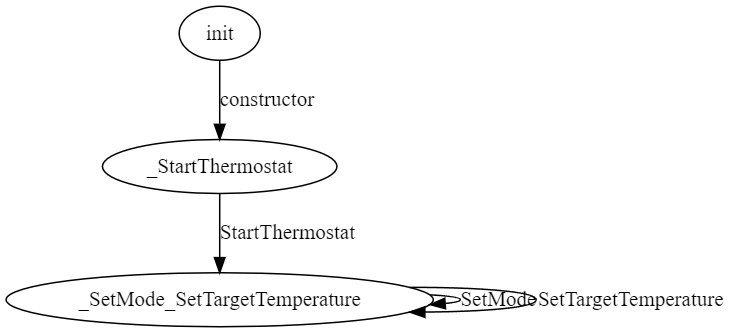
\includegraphics[width=\textwidth]{figs/room-thermostate-epa.png}
        \caption{Enabledness Preserving Abstraction del contrato \texttt{RoomThermostat} }
        \label{fig:room-thermostat-epa}
    \end{subfigure}
\end{figure}

\subsection{Caso \texttt{BoundedStack}}
El siguiente caso que evaluamos fue el ejemplo teórico que expusimos en la sección \ref{sec:subaproximacion}, el contrato \texttt{BoundedStack}, con intención de evidenciar las subaproximaiones realizadas por el algoritmo nuevo.
El código del contrato se encuentra en el fragmento de código \ref{code:solidity-bounded-stack}.
Nos interesa corroborar el comportamiento de ambos algoritmos, si se produce alguna subaproximación, y cuáles.

Lo primero que vimos al evaluar la abstracción generada por el algoritmo alternativo sobre el contrato \texttt{BoundedStack} lo podemos ver en la imagen \ref{fig:buggy-bounded-stack-epa}.
En esa abstracción  podemos ver que faltan algunas de las transiciones presentes en la EPA del contrato, pero además podemos observar que las transiciones por \textcolor{orange}{\texttt{pop}} siempre llevan al estado desde el que se ejecutó el método.
Cuando realizamos esta comparación, esta observación generó bastante confusión, hasta que comprendimos que se debía a un defecto en el código fuente de \texttt{BoundedStack} que no decrementaba la variable \texttt{size} al ejecutar \textcolor{orange}{\texttt{pop}}.
Luego de corregir el defecto, la abstracción generada por el prototipo fue la referenciada en la imagen \ref{fig:bounded-stack-bad-epa}.
Es decir, la misma que elaboramos durante el ejemplo teórico del comportamiento del algoritmo alternativo, y la que evidenciaba la falencia del algoritmo alternativo para este ejemplo.
Decidimos incluir este pequeña caso de un error en el código fuente en lugar de omitirlo para ejemplificar que, a pesar de que quede evidenciado que el algoritmo nuevo genere subaproximaciones de las EPAs en la práctica, las abstracciones generadas pueden seguir resultando útiles a la hora de atrapar errores.

\begin{figure}[H]
    \centering
    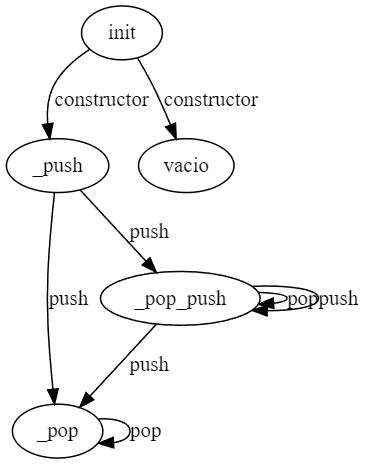
\includegraphics[width=0.45\textwidth]{figs/buggy-bounded-stack-epa.png}
    \caption{Enabledness Preserving Abstraction del contrato \texttt{BoundedStack} con un error que no decrementa el tamaño luego de ejecutar \textcolor{orange}{\texttt{pop}} }
    \label{fig:buggy-bounded-stack-epa}
\end{figure}

A la hora de emplear el algoritmo clásico sobre el contrato, el invariante propuesto fue el siguiente:
\begin{lstlisting}[language=Solidity]
    function invariant() public returns(bool){
        bool result = (size >= 0) && (size <= maxSize);
        result = result && (internal_arr.length == size);
        return result;
    }
\end{lstlisting}

Sin embargo, el prototipo desarrollado con el algoritmo clásico no pudo analizar este contrato satisfactoriamente, sino que terminó el analisis por time out.
Esto se debe a que el paso de restringir las instancias del contrato a aquellas que satisfagan el invariante resultó demasiado difícil para el motor de ejecucion simbólica de Manticore.
Algunos experimentos y análisis intermedios nos hacen creer que se debe a la pobre representación de las variables de tipo \textcolor{cyan}{\texttt{uint256[]}} del mismo.
Esto significó que terminamos el análisis comparando la abstracción generada por el algoritmo alternativo no con la generada por el algoritmo clásico, sino con una EPA producida manualmente.

\section{Comparación en tiempo de ejecución entre el algoritmo clásico y el alternativo}
Otra hipótesis generada durante el desarrollo del algoritmo alternativo fue que el evitar la ejecución de los invariantes mejoraría el tiempo de ejecución.
Esto se debe a que los invariantes, comparados con las precondiciones de los métodos externos, son propiedades relativamente complejas que además pueden hablar sobre el estado de variables internas de tipos complejos como arrays, mappings, etc.
Para evaluar esta hipótesis estudiamos el tiempo de ejecución empleado por los prototipos que implementan el algoritmo alternativo y el clásico en Manticore sobre algunos de los contratos pertenecientes al benchmark Microsoft Azure Blockchain Workbench \cite{azure-benchmark}.

Ya que este mismo benchmark había sido utilizado por Godoy et al. en 2022 \cite{predicate-abstraction-for-smart-contract-validation}, a la hora de experimentar contamos con EPAs de todos los contratos involucrados, por lo que además pudimos usarlas para corroborar la correctitud de las abstracciones generadas.
Los experimentos fueron realizados ejecutando ambos prototipos sobre cada contrato cinco veces y luego tomando el promedio del tiempo total de ejecución.
Todas las mediciones fueron realizadas en una máquina en una máquina \textcolor{red}{\textbf{DESCRIPCION MAQUINA}}.

En la figura \ref{fig:classic-vs-alternativo} podemos ver los resultados del experimento realizado.
Las mediciones fueron solo realizadas para los contratos \texttt{DefectiveComponentCounter}, \texttt{RoomThermostat}, \texttt{BasicProvenance} y \texttt{SimpleMarketplace} porque como podemos ver el tiempo de ejecución de la implementación del algoritmo clásico nunca fue menor a diez horas.
A pesar de que en todos los contratos analizados podamos ver una diferencia significativa al emplear el algoritmo alternativo, es importante destacar que los tiempos de ejecución de esta técnica aún se mantuvieron muy altos.
La mejora en tiempo parecería ser relativamente constante a lo largo de los cuatro contratos analizados, habiendo tardado el algoritmo alternativo alrededor de diez horas menos que el clásico.
Esta diferencia cercana a constante posiblemente se deba a que todos los contratos eran muy simples (recordemos la baja cantidad de métodos externos en \texttt{SimpleMarketplace} y \texttt{RoomThermostat}), por lo que no se pudo observar la diferencia en comportamiento que habría en contratos más complejos.

\begin{figure}[h]
    \centering
    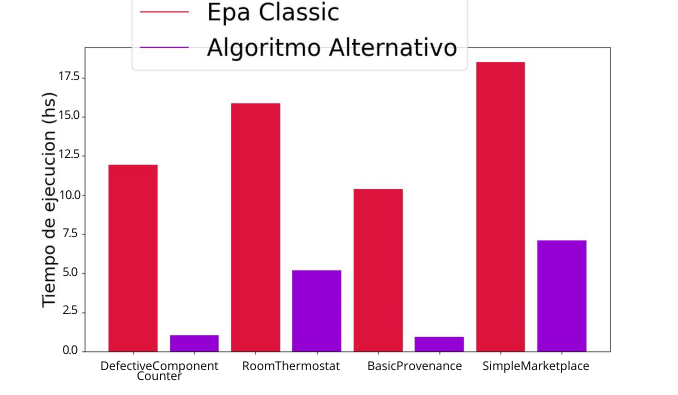
\includegraphics[width=0.65\textwidth]{figs/classic_vs_alternativo.png}
    \caption{Tiempo promediado para 5 ejecuciones (en horas) de la generación de abstracciones del prototipo que implementa el algoritmo alternativo y el algoritmo clásico}
    \label{fig:classic-vs-alternativo}
\end{figure}

A pesar de que la mejora del algoritmo alternativo frente al clásico fuese tan grande, los valores obtenidos con el algoritmo alternativo siguieron sin resultar razonables.
Si observamos los valores obtenidos, el tiempo de cómputo en promedio fue de entre media hasta casi ocho horas, lo que no resulta aplicable para un usuario de la herramienta que pretende generar las abstracciones en tiempo real.
Por este motivo decidimos realizar los experimentos que mostraremos a continuación, en los que buscamos conseguir mejoras en el tiempo de ejecución o claridad en la razón de que tarde tanto.


\section{Evaluación más detallada del tiempo de ejecución del algoritmo alternativo}
Para mejorar el tiempo de ejecución del prototipo buscamos identificar en qué partes del análisis era que se consumía la mayor parte del tiempo empleado.
Lo primero que hicimos fue identificar ``etapas'' en el algoritmo alternativo que pudimos diferenciar para medir el tiempo empleado en cada una de ellas.
Por otro lado analizamos el código fuente de Manticore y diferenciamos en distintos niveles de abstracción las funcionalidades que estábamos usando.

La separación de la ejecución del algoritmo en etapas la hicimos en estas dos:
\begin{enumerate}
    \item La ejecución simbólica de los métodos
    \item La solución de queries de satisfacibilidad sobre las transiciones en la EPA
\end{enumerate}
Donde notoriamente incluimos el desplegado simbólico del contrato en la misma etapa que la ejecución de los métodos.
Refiriéndonos al algoritmo alternativo, podemos ver que este alterna entre estas dos etapas.
Nos resulta de interés ver cuál, si alguna, consume la mayor parte del tiempo de ejecución.

A continuación indicamos cuál fue la división en niveles de abstracción que hicimos de las funcionalidades de Manticore.
En particular, por como es la arquitectura de multithreading y \textbf{\texttt{workers}} de Manticore, solo pudimos hacer esta distinción en los métodos relacionados a la resolución de valores simbólicos.
La manera en la que se realizaba la ejecución simbólica y la generación de las path conditions era demasiado dependiente de objetos creados dinámicamente como para poder ser analizada de la misma manera.
\begin{enumerate}
    \item \textbf{Nivel Externo}\footnote{En el momento de realizar las mediciones, los valores para este nivel se registraron bajo el nombre de  ``Nivel 3''} : utilizado para medir el tiempo que consumían las funciones de la API de manticore que nuestro prototipo llamaba directamente.
          La única función cuyo tiempo medimos en este nivel fue \texttt{generateTestCases}.
    \item \textbf{Nivel \texttt{state}} : Utilizado en las funciones del módulo \textbf{\texttt{state}} que identificamos que eran llamadas.
          Los métodos registrados bajo este nivel fueron \texttt{can\_be\_true} y \texttt{solve\_\allowbreak one\_\allowbreak n\_\allowbreak batched}.
    \item \textbf{Nivel SMT solver} : Utilizado alrededor de cada llamado directo al SMT solver en los métodos del módulo \textbf{\texttt{smtlib}}.
          Los métodos registrados bajo este nivel fueron \texttt{\_is\_sat}, \texttt{\_get\_value} y \texttt{\_\_get\_value\_all}.
\end{enumerate}
Cada uno de los métodos fue modificado para medir el tiempo empleado entre el principio y el fin de la zona delimitada de interés.
Por ejemplo, en el fragmento de códgio \ref{code:getvalueall-modification} podemos ver los cambios introducidos en el método \texttt{\_\_get\_value\_all} del \textbf{Nivel SMT solver} para registrar el tiempo.

\begin{lstlisting}[language=Python,
    label={code:getvalueall-modification},
    caption={Método \texttt{\_\_get\_value\_all} del modulo \textbf{\texttt{smtlib}} modificado para registrar el tiempo empleado por la llamada al SMT solver. El resaltado indica las líneas agregadas para registrar el tiempo.},
    captionpos=b]
def __getvalue_all(self, expressions_str: List[str], is_bv: List[bool]) -> Dict[str, int]:
    (*@| \hl{start = time.time()} |@*)
    all_expressions_str = " ".join(expressions_str)
    self._smtlib.send(f"(get-value ({all_expressions_str}))")
    ret_solver: Optional[str] = self._smtlib.recv()
    (*@| \hl{print}|@*)(f"(level _getvalue_all_z3_call) took {time.time()- start} seconds")
    assert ret_solver is not None
    return_values = re.findall(RE_GET_EXPR_VALUE_ALL, ret_solver)
    
    return {value[0]: _convert(value[1]) for value in return_values}
\end{lstlisting}

De  entre los métodos a los que les registramos el tiempo de ejecución, sabíamos que los métodos en \textbf{Nivel Externo} solo eran ejecutados cuando el prototipo implementado los llamaba explícitamente.
Por otro lado, los métodos en \textbf{Nivel \texttt{state}} eran métodos que a veces eran llamados desde la implementación directamente, pero además eran ejecutados como métodos internos de otros procesos durante el análisis.
Por último, los métodos del \textbf{Nivel SMT solver} eran ejecutados en diversos momentos del análisis.

Una vez hecha esta separación en etapas del algoritmo y niveles de abstracción, medimos el tiempo total en promedio empleado por cada etapa y cada nivel de abstracción.
Para esto, al igual que antes, analizamos el rendimiento en los contratos \texttt{DefectiveComponent\allowbreak Counter}, \texttt{RoomThermostat}, \texttt{BasicProvenance}, \texttt{SimpleMarketplace} y \texttt{HelloBlockchain} del benchmark Microsoft Azure Blockchain Workbench \cite{azure-benchmark}.
Por otro lado, además, calculamos para cada uno de los niveles de abstracción la cantidad de veces que este mismo fue registrado y el tiempo total empleado.
Esto fue para intentar percibir discrepancias entre los niveles que espérabamos que consumieran la mayoría del tiempo y lo que pudiéramos medir.

\subsection{Resultados}

\begin{figure}
    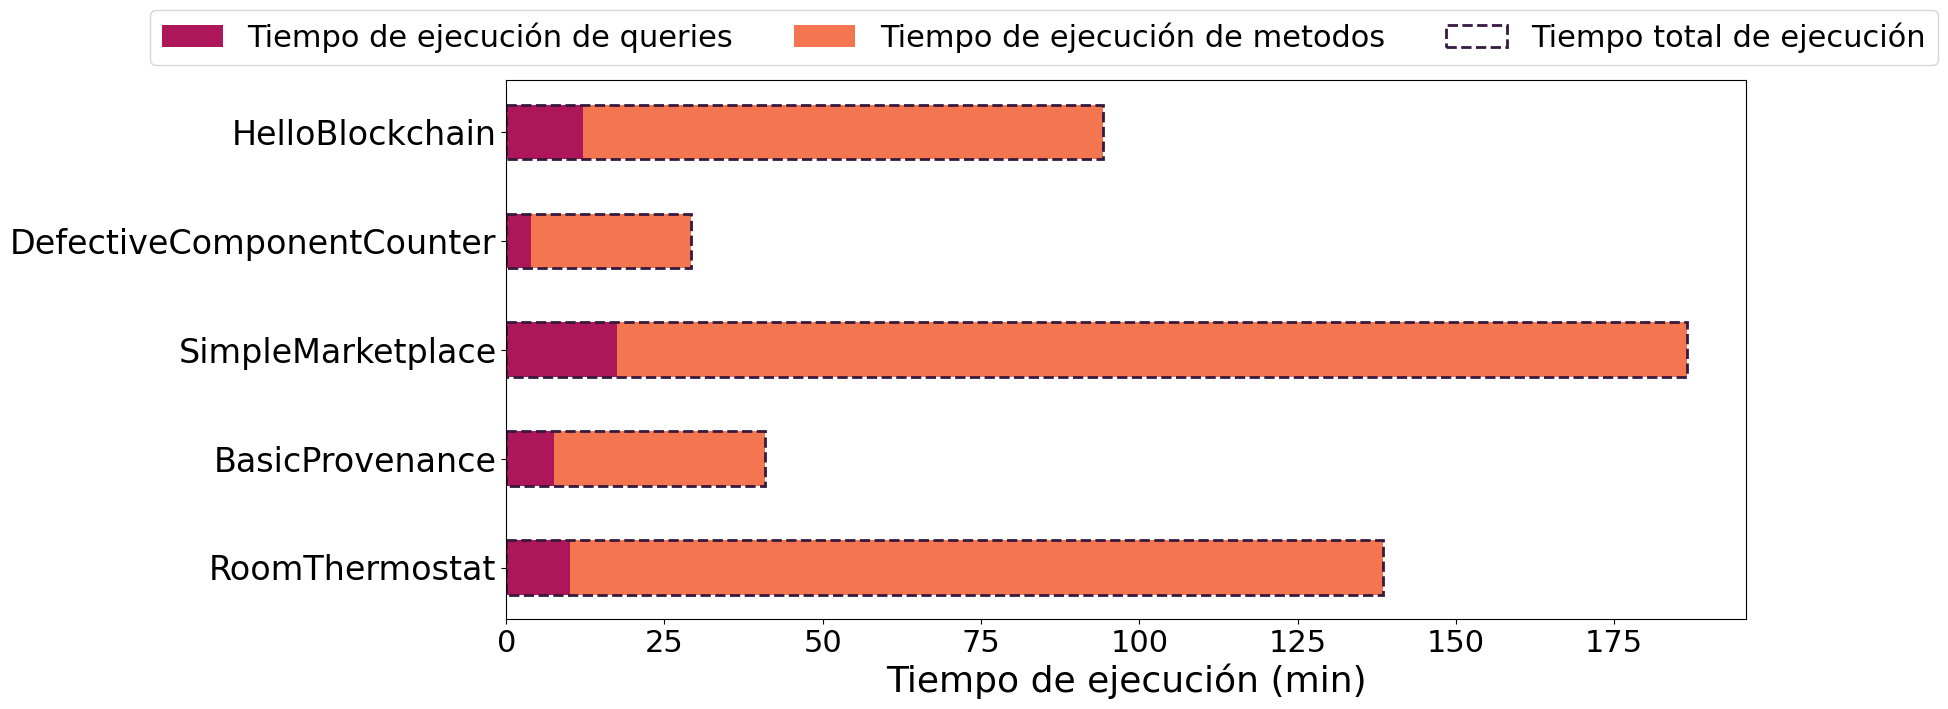
\includegraphics[width=\textwidth]{figs/categories-bar-graph.png}
    \caption{Proporción del tiempo de ejecución promediado entre 5 (en horas) del algoritmo alternativo.
        En naranja el tiempo empleado por la ejecución simbólica de los métodos, en violeta por la resolución de queries de predicados y en líneas punteadas el tiempo total (medido) empleado por el algoritmo.}
    \label{fig:tiempo-categorias}
\end{figure}

En la figura \ref{fig:tiempo-categorias} podemos ver las mediciones obtenidas sobre el tiempo empleado por las dos etapas del algoritmo.
Se ve que la gran mayoría del tiempo empleado durante la generación de EPAs con el algoritmo involucrado fue consumido por la ejecución simbólica de los métodos.
La resolución de predicados para consultar por la presencia de transiciones en la EPA, en cambio, fue comparativamente pequeña.
Por ejemplo, para el contrato \texttt{HelloBlockchain}, podemos ver que a pesar que el tiempo total promedió cercano los 94 minutos, la etapa de resolución de queries demoró tan sólo valores cercanos a los 12 minutos.
Por otro lado, la suma del tiempo empleado en promedio por ambas etapas resulta a simple vista idéntico al tiempo total promedio que se pudo medir, por lo que tampoco observamos un consumo inusualmente alto de tiempo por algún otro aspecto del análisis sin considerar.

En la tabla \ref{tab:performance} podemos ver un caso de estudio de los resultados obtenidos en las mediciones del tiempo empleado en cada nivel de abstracción de los métodos de Manticore.
Nos limitamos a analizar los valores obtenidos para el contrato \texttt{HelloBlockchain} para no mezclar los valores de distintos contratos, debido a que nos interesa señalar las relaciones entre los valores para algunos de los métodos.
Haciendo memoria sobre el análisis de la figura \ref{fig:tiempo-categorias}, podemos ver que los aproximadamente 713 segundos empleados por el método \texttt{generateTestCases}, que es el más externo de todos, representan casi la totalidad (12 minutos) del tiempo empleado por la etapa de solución de queries del programa.
De hecho, los métodos \texttt{solve\_one\_n\_batched} y \texttt{get\_value\_in\_batch}, que pertenecen a un nivel de abstracción menor, siguen siendo responsables por la mayoría del tiempo empleado (y si observamos el número de veces que cada uno fue llamado, a fines del análisis que estamos haciendo ambos métodos resultan prácticamente iguales).
Sin embargo, al realizar el salto a los métodos de \textbf{Nivel SMT solver}, vemos que comparativamente estos casi ni aportaron al tiempo empleado.
Los tres métodos \texttt{\_getvalue\_all}, \texttt{\_is\_sat} y \textt{\_getvalue}, todos llamados de manera directa por los métodos del nivel superior, apenas aportan 4 segundos de los 12 minutos involucrados.

De aquí podemos intentar obtener dos conclusiones.
O bien las llamadas al SMT solver funcionan de una manera asincrónica, que no pudimos capturar en nuestras mediciones, o bien en efecto la mayoría del tiempo consumido por consultas a Manticore es empleado no en tiempo de procesamiento del SMT solver, sino en alguna etapa de la aplicación misma (que no fuimos capaces de medir).
Considerando ya que la mayor parte del tiempo de ejecución de la aplicación fue consumido por la etapa de ejecución simbólica, y no por la de resolución de queries, es posible que el preprocesamiento de las condiciones simbólicas de Manticore, construido durante la etapa de ejecución simbólica, sea extraordinariamente complejo y por ende caro en tiempo de ejecución.
Además, un rudimentario y primer análisis del código involucrado sugiere que los llamados realizados al SMT solver son completamente sincrónicos, aunque no se pudo realizar un experimento para corroborar ninguna de estas dos hipótesis.


% Define custom colors
\definecolor{color1}{rgb}{0.9, 0.9, 0.9} % Light gray
\definecolor{color2}{rgb}{0.8, 0.8, 0.8} % Medium gray
\definecolor{color3}{rgb}{0.7, 0.7, 0.7} % Dark gray

\begin{table}[ht]
    \centering
    \begin{tabular}{l @{\hskip 30pt} r @{\hskip 30pt} r}
        \toprule
        \textbf{Método de Manticore}                      & \textbf{Número de llamados} & \textbf{Tiempo empleado (s)} \\
        \midrule
        \rowcolor{color1} \texttt{\_getvalue}             & 6                           & 0.00458                      \\
        \rowcolor{color1} \texttt{\_is\_sat}              & 92                          & 0.52989                      \\
        \rowcolor{color2} \texttt{state.can\_be\_true}    & 24                          & 0.13410                      \\
        \rowcolor{color1} \texttt{\_getvalue\_all}        & 32                          & 3.73966                      \\
        \rowcolor{color2} \texttt{get\_value\_in\_batch}  & 54                          & 712.47606                    \\
        \rowcolor{color2} \texttt{solve\_one\_n\_batched} & 54                          & 713.05950                    \\
        \rowcolor{color3} \texttt{generateTestCases}      & 3                           & 713.35846                    \\
        \bottomrule
    \end{tabular}
    \caption{Tiempo empleado por los métodos de Manticore involucrados en las queries por transiciones en la EPA para el contrato \texttt{HelloBlockchain}. En el color más oscuro los métodos del \textbf{Nivel Externo}, en el color intermedio los del \textbf{Nivel \texttt{state}} y en el más claro los del \textbf{Nivel SMT solver}.}
    \label{tab:performance}
\end{table}
